\documentclass[specialist, 12pt, 
subf, %draft,
href, colorlinks=true,
substylefile = spbu.rtx,
]{disser}

%draft
\usepackage[
a4paper, mag=1000, includefoot,
left=3cm, right=1.5cm, top=2cm, bottom=2cm, headsep=1cm, footskip=1cm
]{geometry}

\usepackage{float}
\usepackage[T2A]{fontenc}
\usepackage[utf8]{inputenc}
\usepackage[english,russian]{babel}
\ifpdf\usepackage{epstopdf}\fi
\usepackage{cmap}
\usepackage{graphicx}
\usepackage{multicol,caption}
\usepackage[final]{listings}
\usepackage[ruled,linesnumbered]{algorithm2e}
\usepackage{amsmath}
\usepackage{amsthm}
\usepackage{amssymb}
\usepackage{amsfonts}
\usepackage{listings}
\usepackage{xcolor}
\usepackage{wrapfig}
%\usepackage{subfigure}
%\usepackage{longtable}
\usepackage{array}
%\usepackage{bbold}
\usepackage{subcaption}
%\setcounter{MaxMatrixCols}{48}
\usepackage{resizegather}
\usepackage{hyperref}

%\usepackage{algorithm}
%\usepackage{algpseudocode}
\usepackage[]{algorithm2e}
% Перевод плагина
\SetKwInput{KwData}{Исходные параметры}
\SetKwInput{KwResult}{Результат}
\SetKwInput{KwIn}{Входные данные}
\SetKwInput{KwOut}{Выходные данные}
\SetKwIF{If}{ElseIf}{Else}{если}{тогда}{иначе если}{иначе}{конец условия}
\SetKwFor{While}{до тех пор, пока}{выполнять}{конец цикла}
\SetKw{KwTo}{от}
\SetKw{KwRet}{возвратить}
\SetKw{Return}{возвратить}
\SetKwBlock{Begin}{начало блока}{конец блока}
\SetKwSwitch{Switch}{Case}{Other}{Проверить значение}{и выполнить}{вариант}{в противном случае}{конец варианта}{конец проверки значений}
\SetKwFor{For}{цикл}{выполнять}{конец цикла}
\SetKwFor{ForEach}{для каждого}{выполнять}{конец цикла}
\SetKwRepeat{Repeat}{повторять}{до тех пор, пока}
\SetAlgorithmName{Алгоритм}{алгоритм}{Список алгоритмов}



\let\vec=\mathbf
\widowpenalty=10000
\clubpenalty=10000
\setcounter{tocdepth}{2}


\graphicspath{{fig/}}


\newtheorem{proposition}{Утверждение} 
\newtheorem{definition}{Определение} 
\newtheorem{theorem}{Теорема} 
\newtheorem{investigation}{Следствие} 
\newtheorem{designation}{Обозначение} 
\newtheorem{remark}{Замечание}
\newtheorem{example}{Пример}

\DeclareMathOperator{\diag}{diag}
\DeclareMathOperator{\spn}{span}
\DeclareMathOperator{\rnk}{rank}
\DeclareMathOperator{\dist}{dist}
\DeclareMathOperator{\sign}{sign}
\begin{document} 
	
	\lstset{ 
		basicstyle=\ttfamily\footnotesize, % the size of the fonts that are used for the code 
		numbers=left, % where to put the line-numbers 
		numberstyle=\footnotesize, % the size of the fonts that are used for the line-numbers 
		stepnumber=1, % the step between two line-numbers. If it's 1, each line 
		% will be numbered 
		numbersep=8pt, % how far the line-numbers are from the code 
		language=R} 
	\institution{ 
		Санкт-Петербургский государственный университет \\ 
		Прикладная математика и информатика \\ 
		Статистическое моделирование
	} 
	
	
	\title{Конспект} 
	
	% Тема 
	\topic{\normalfont\scshape % 
	Нейронные сети. Общая структура (особый класс функций для оптимизации). Back propagation как вычислительный подход} 
	
	% Автор 
	\author{Третьякова Александра, Волканова Маргарита, Федоров Никита} 
	

	
	% Город и год 
	\city{Санкт-Петербург}
	\date{2019}
	
	
	
	\maketitle
	%\tableofcontents
	
	%\intro
	
	\section{Постановка задачи. Аппроксимация особым классом функций}
	
	Пусть $X$ --- множество объектов, $Y$ --- множество ответов. Пусть есть обучающая выборка $X^n = (x_i, y_i)_{i=1}^{n},$ $x_i \in \mathbb{R}^p$. Обозначим $(x^1,\ldots,x^p)\in \mathbb{R}^p$ --- вектор признаков объекта $x\in X$. Рассмотрим следующую задачу построения предсказывающей модели:
	\begin{equation*}
	Q(a, X^n) = \frac{1}{n} \sum_{i=1}^{n} \mathcal{L}(a,x_i,y_i) \rightarrow \min_w,
	\end{equation*}
	где алгоритм $a$ зададим следующим образом (рассмотрим особый класс функций):
	\begin{equation*}
	a(x, w) = \sigma( \langle w,x \rangle ) = \sigma\left(\sum_{j=1}^{p} w_j x^j - w_0 \right),
	\end{equation*}
	где $w_k \in \mathbb{R}$, $k=0,\ldots,p$ --- параметры; 
	$\sigma: \mathbb{R} \rightarrow  \mathbb{R} $ --- функция активации;
	$\mathcal{L}(a,x_i,y_i)$ --- функция потерь, $i=1,\ldots,n$. Такой класс функций включает в себя, например, линейную классификацию и линейную регрессию.
	
	Задача классификации. Пусть $Y=\{+1,-1\}$. Если $\sigma (z)=\sign (z)$, то $a(x,w)$ --- линейный классификатор, и задача выглядит следующим образом: 
	
	\begin{equation*}
	Q(w, X^{n})=\sum_{j=1}^{n} \mathcal{L} \left( a(x_j ,w), y_j \right) = \sum_{j=1}^{n} [y_j \langle w,x_j \rangle  < 0] \rightarrow \min_{w}.
	\end{equation*}
	
	Задача регрессии. Пусть $Y=\mathbb{R}$. Если взять $\sigma(z)=z$, то получим многомерную линейную регрессию:
	\begin{equation*}
	Q(w, X^{n})=\sum_{j=1}^{n} \mathcal{L} \left( a( x_j,w ), y_j \right)=\sum_{j=1}^{n}\left( \langle w,x_j \rangle  -y_j \right)^2 \rightarrow \min_{w}.
	\end{equation*}
	
	\section{Модель нейрона МакКаллока-Питтса}
	
	Рассмотренный класс функций удобно представить схематически (рисунок~\ref{neur}). Такой класс функций является простейшей математической моделью нервной клетки --- нейрона. Схема нейрона представлена на рисунке~\ref{cell}.
	
	\begin{figure}[h]
		\begin{center}
			\begin{minipage}[h]{0.5\linewidth}
				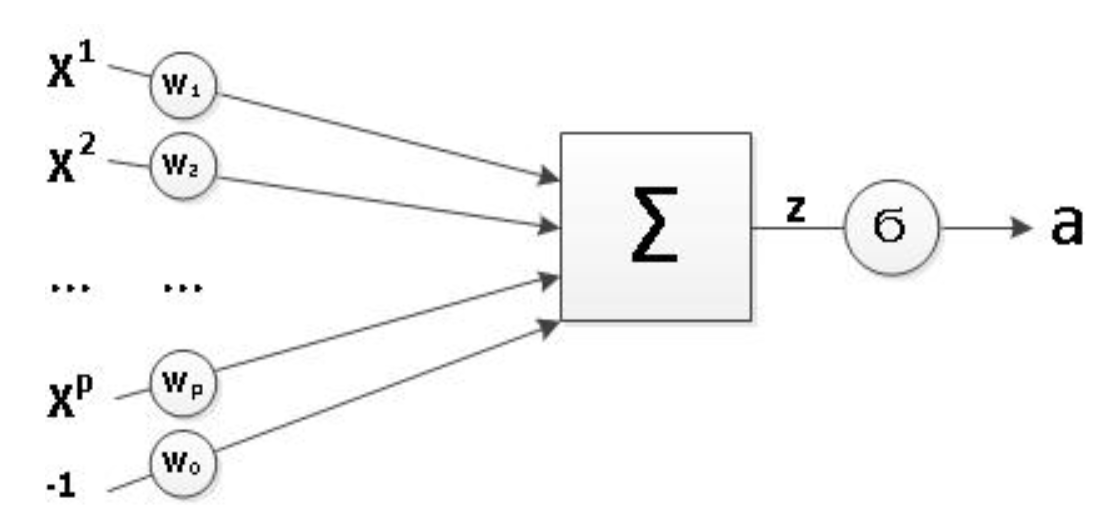
\includegraphics[width=1\linewidth]{neur1}
				\caption{Схема особого класса функций.} 
				\label{neur} 
			\end{minipage}
			\hfill
			\begin{minipage}[h]{0.45\linewidth}
				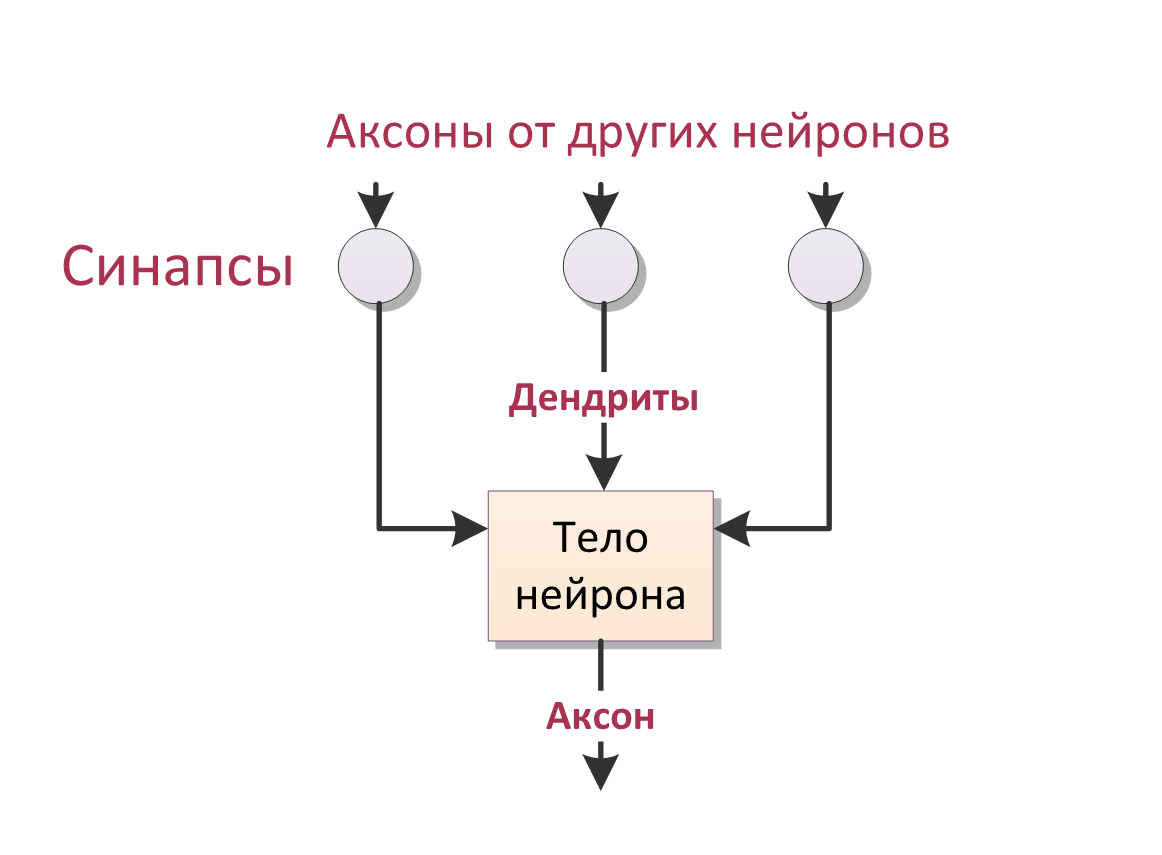
\includegraphics[width=1\linewidth]{cell}
				\caption{Схема нервной клетки.}
				\label{cell}
			\end{minipage}
		\end{center}
	\end{figure}


Нервную клетку можно рассматривать как устройство, которое принимает заряды величиной $x^j$ от $p$ входов --- синапсов, примыкающих к ее дендритам. Поступающие заряды складываются с весами $w_j$. Если суммарный заряд превышает порог активации $w_0$, то нейрон возбуждается и выдает на выходе $+1$, иначе выдается $-1$. Модель нейрона МакКаллока-Питтса эквивалентна пороговому линейному классификатору. 
	
$x^j \in \mathbb{R}^n$ называются числовыми входами, $w_j\in\mathbb{R}$ --- весовые коэффициенты (синаптические веса), $\sigma(z)$ --- функция активации, $w_0$ --- порог активации. Смысл термина "порог активации"$~$ становится понятен, если взять конкретную функцию активации $\sigma(z)$, к примеру, выпрямитель $ReLU(p) = \max (0,p)$.
	
	\section{Аппроксимация функций особым классом}
	
	Хочется узнать, любая ли функция может быть аппроксимирована введенным нами особым классом функций.
	
	\subsection{Булевы функции в виде нейронов}
	
	Рассмотрим простейшие булевы функции --- НЕ, И, ИЛИ. Каждая из этих функций может быть представлена в виде одного нейрона. 
	\begin{enumerate}
		\item Логическая операция НЕ может быть представлена в виде $\lnot x^1 = [-x^1+\frac{1}{2}>0]$. На рисунке~\ref{bool1} представлен нейрон, реализующий эту операцию.
		\begin{figure}[h]
			\begin{center}
				\begin{minipage}{0.5\linewidth}
					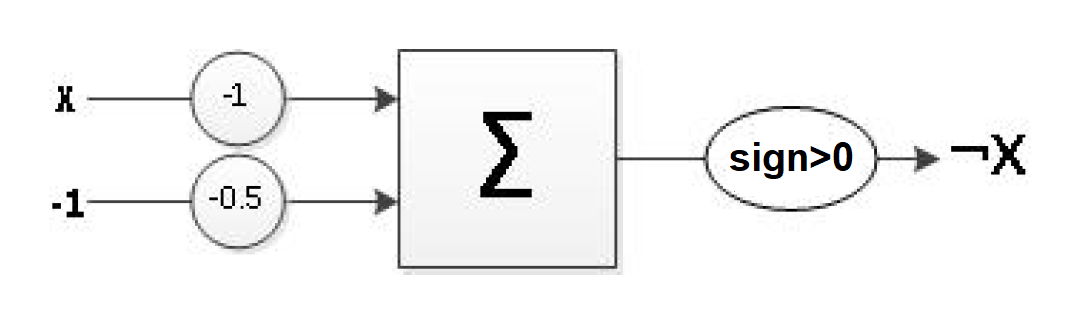
\includegraphics[width=250pt, height=70pt]{boolean1}
					\caption{Представление логической операции НЕ в виде нейрона.}
					\label{bool1}
				\end{minipage}
			\end{center}
		\end{figure}
		\item Логические операции ИЛИ, И могут быть представлены в таком виде: $x^1 \lor x^2 = [x^1+x^2 -\frac{1}{2}>0]$ и $x^1 \wedge x^2 = [x^1+x^2 -\frac{3}{2}>0]$. На рисунке~\ref{bool2} представлены нейроны, реализующие эти булевы функции.
		\begin{figure}[h]
			\begin{center}
				\begin{minipage}{0.85\linewidth}
					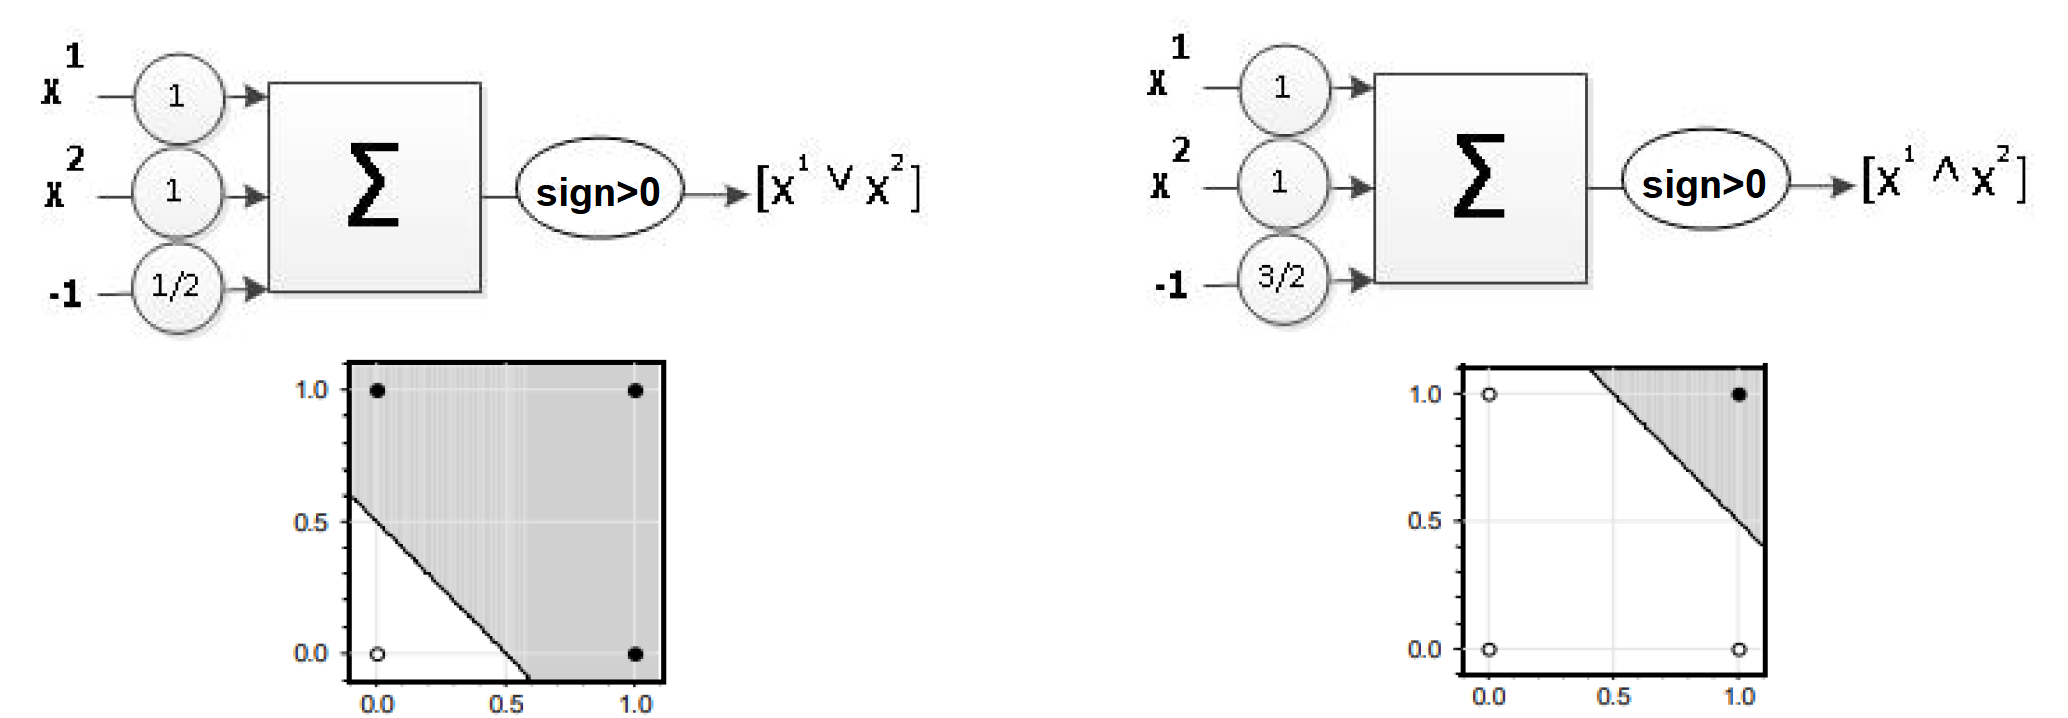
\includegraphics[width=450pt, height=150pt]{boolean2}
					\caption{Представление логических операций ИЛИ и И в виде нейронов.}
					\label{bool2}
				\end{minipage}
			\end{center}
		\end{figure}
	   
	   \item Задача "исключающего ИЛИ". Такая операция не может быть реализована одним нейроном с двумя входами $x^1$ и $x^2$. Возможны два варианта решения такой задачи. 
	   
	   \begin{itemize}
	 \item  Первый вариант --- пополнить пространство признаков, добавить нелинейное преобразование исходных признаков. Например, если добавить произведение исходных признаков, тогда нейрон будет строить уже не линейную, а полиномиальную разделяющую поверхность. Таким образом, мы перейдем к спрямляющему пространству признаков. Функцию "исключающего ИЛИ"$~$ можно представить в виде $x^1 \oplus x^2 = [x^1+x^2 -2x^1x^2-\frac{1}{2}>0]$, схема нейрона представлена на рисунке~\ref{bool3}.
	   
	   		\begin{figure}[h]
	   	\begin{center}
	   		\begin{minipage}{0.75\linewidth}
	   			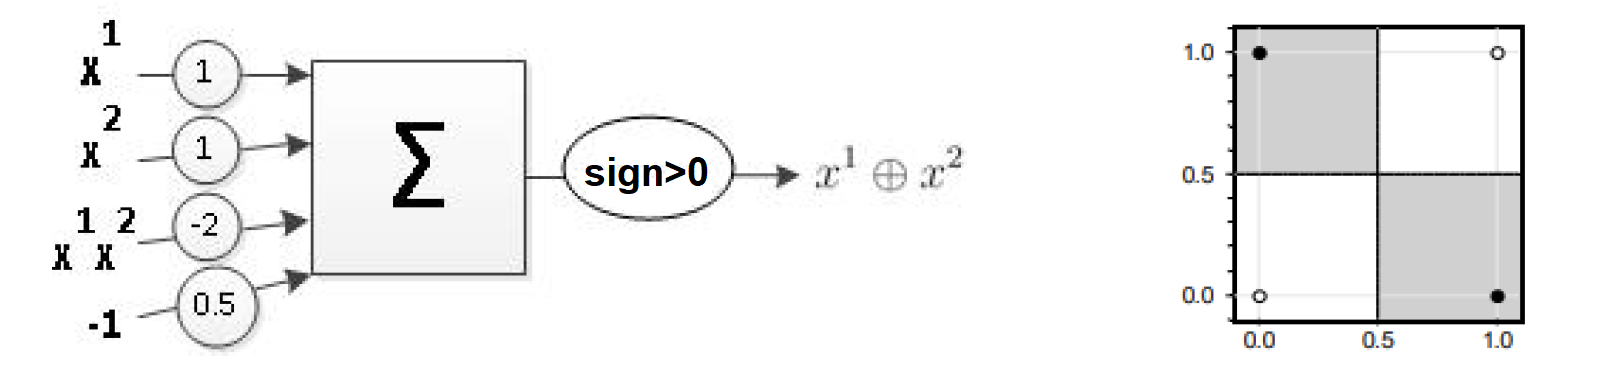
\includegraphics[width=350pt, height=85pt]{boolean3}
	   			\caption{Представление логической операции "исключающее ИЛИ" $~$ в виде одного нейрона.}
	   			\label{bool3}
	   		\end{minipage}
	   	\end{center}
	   \end{figure}
   
   \item Второй вариант --- построить композицию из нескольких нейронов. Например, "исключающее ИЛИ"$~$ можно представить в таком виде: $x^1 \oplus x^2 = [\lnot((x^1\lor x^2) - (x^1 \wedge x^2))>0]$. Получаем суперпозицию нейронов --- нейронную сеть (рисунок~\ref{bool4}).
   
      \begin{figure}[h]
   	\begin{center}
   		\begin{minipage}{0.75\linewidth}
   			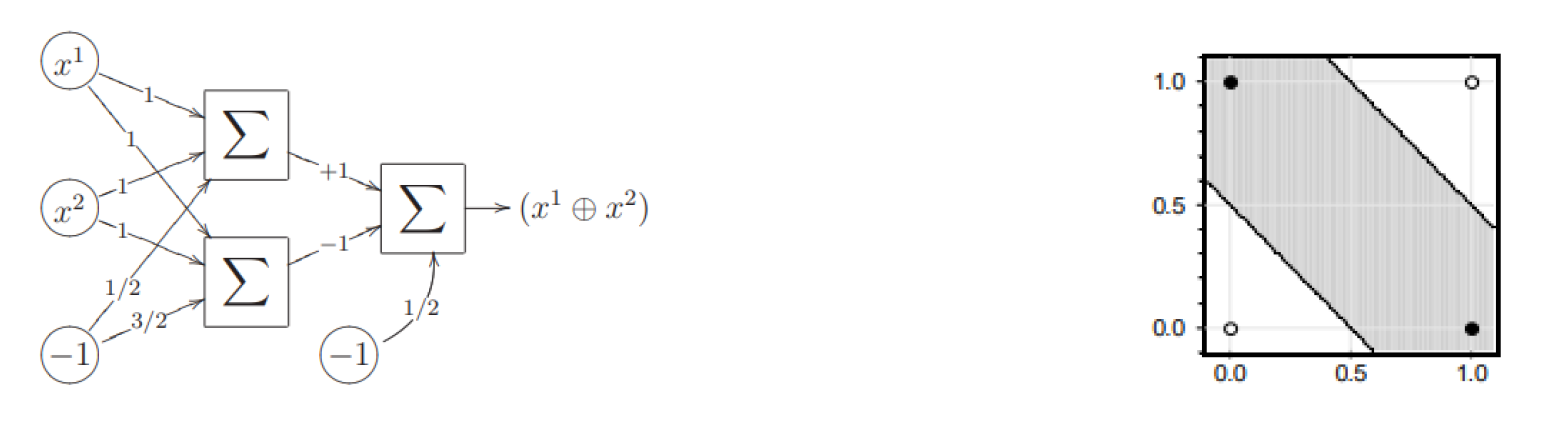
\includegraphics[width=350pt, height=85pt]{boolean4}
   			\caption{Представление логической операции "исключающее ИЛИ" $~$ в виде суперпозиции нейронов.}
   			\label{bool4}
   		\end{minipage}
   	\end{center}
   \end{figure}
   
	\end{itemize}
	\end{enumerate}
	
	\subsection{Аппроксимация функций суперпозицией нейронов}
	
	Возникает вопрос --- насколько богатый класс функций может быть реализован нейроном? 

\begin{theorem}[Цыбенко, 1989]
	Пусть $\sigma(x)$ --- непостоянная, ограниченная и монотонно возрастающая непрерывная функция; $C(I_{p_0})$ --- множество непрерывных функций на $[0,1]^{p_0}$.
	
	Тогда $\forall f \in C(I_{p_0})$ и $\forall \varepsilon > 0$  $\exists ~p_1 \in \mathbb{Z}$ и  $\alpha_i$, $b_i$, $w_{ij} \in \mathbb{R}$, $i=1,\ldots,p_1$, $j=1,\ldots, p_0$, такие что для любого $x=(x^1, \ldots, x^{p_0}) \in I_{p_0}$ выполняется
		\begin{equation*}
	| F(x^1, \ldots, x^{p_0}) - f(x^1, \ldots, x^{p_0})| < \varepsilon,
		\end{equation*}
	где  \begin{equation*}
	F(x^1, \ldots, x^{p_0})=\sum_{i=1}^{p_1} \alpha_i \, \sigma \left(\sum_{j=1}^{p_0} w_{ij} x^j + b_i   \right).
\end{equation*}
\end{theorem}	

Из этой теоремы можно сделать вывод, что любую непрерывную функцию можно приблизить нейронной сетью с любой желаемой точностью. А также, что для этой сети требуется один скрытый слой и одна нелинейная функция активации. 

\begin{remark}
	Верно следующее:
	\begin{enumerate} 
		\item Двухслойная сеть в $\{0,1\}^n$ позволяет реализовать любую булеву функцию. 
		\item Двухслойная сеть в $\mathbb{R}^n$ позволяет реализовать любой выпуклый многогранник. 
		\item Трехслойная сеть в $\mathbb{R}^n$ позволяет отделить любую многогранную область, не обязательно выпуклую и не обязательно связную. 
		\item С помощью линейных операций и одной нелинейной функции активации можно приблизить любую непрерывную функцию с любой точностью. 
	\end{enumerate}
\end{remark}

В качестве функций активации чаще всего используются следующие функции:
\begin{itemize}
	\item Сигмоидная функция: $\sigma(z) = \frac{1}{1+e^{-a\,z}}$, $a \in \mathbb{R}$;
	
	\item Softmax: $SM_i(z)  = \frac{e^{z_i}}{\sum_{k=1}^{K}e^{z_k}}$;
	\item Гиперболический тангенс: $\sigma(z) = \frac{e^{a\,z} - e^{-a\,z}}{e^{a\,z} + e^{-a\,z}}$, $a \in \mathbb{R}$;
	\item Выпрямитель: $ReLU(p) = \max (0,p)$;
\end{itemize}
Последняя чаще всего используется для нейронных сетей с большим количеством слоев.



\section{Алгоритм обратного распространения ошибки BackProp}


Рассмотрим для удобства двухслойную нейронную сеть. Пусть $Y = \mathbb{R}^M$. Все приведенные ниже рассуждения можно будет обобщить на произвольное количество слоев. Пусть выходной слой состоит из $M$ нейронов с функциями активации $\sigma_m$ и выходами $a^m, m = 1,\ldots,M$. Перед ним находится скрытый слой из $H$ нейронов с функциями активации $\sigma_h$ и выходами $u^h, h = 1, \ldots,H$. Веса синаптических связей между $h$-м нейроном скрытого слоя и $m$-м нейроном выходного слоя будем обозначать через $w_{hm}$. Схема описанной нейронной сети представлена на рисунке~\ref{neuralnetwork}.

\begin{figure}[h]
	\begin{center}
	\begin{minipage}{0.85\linewidth}
		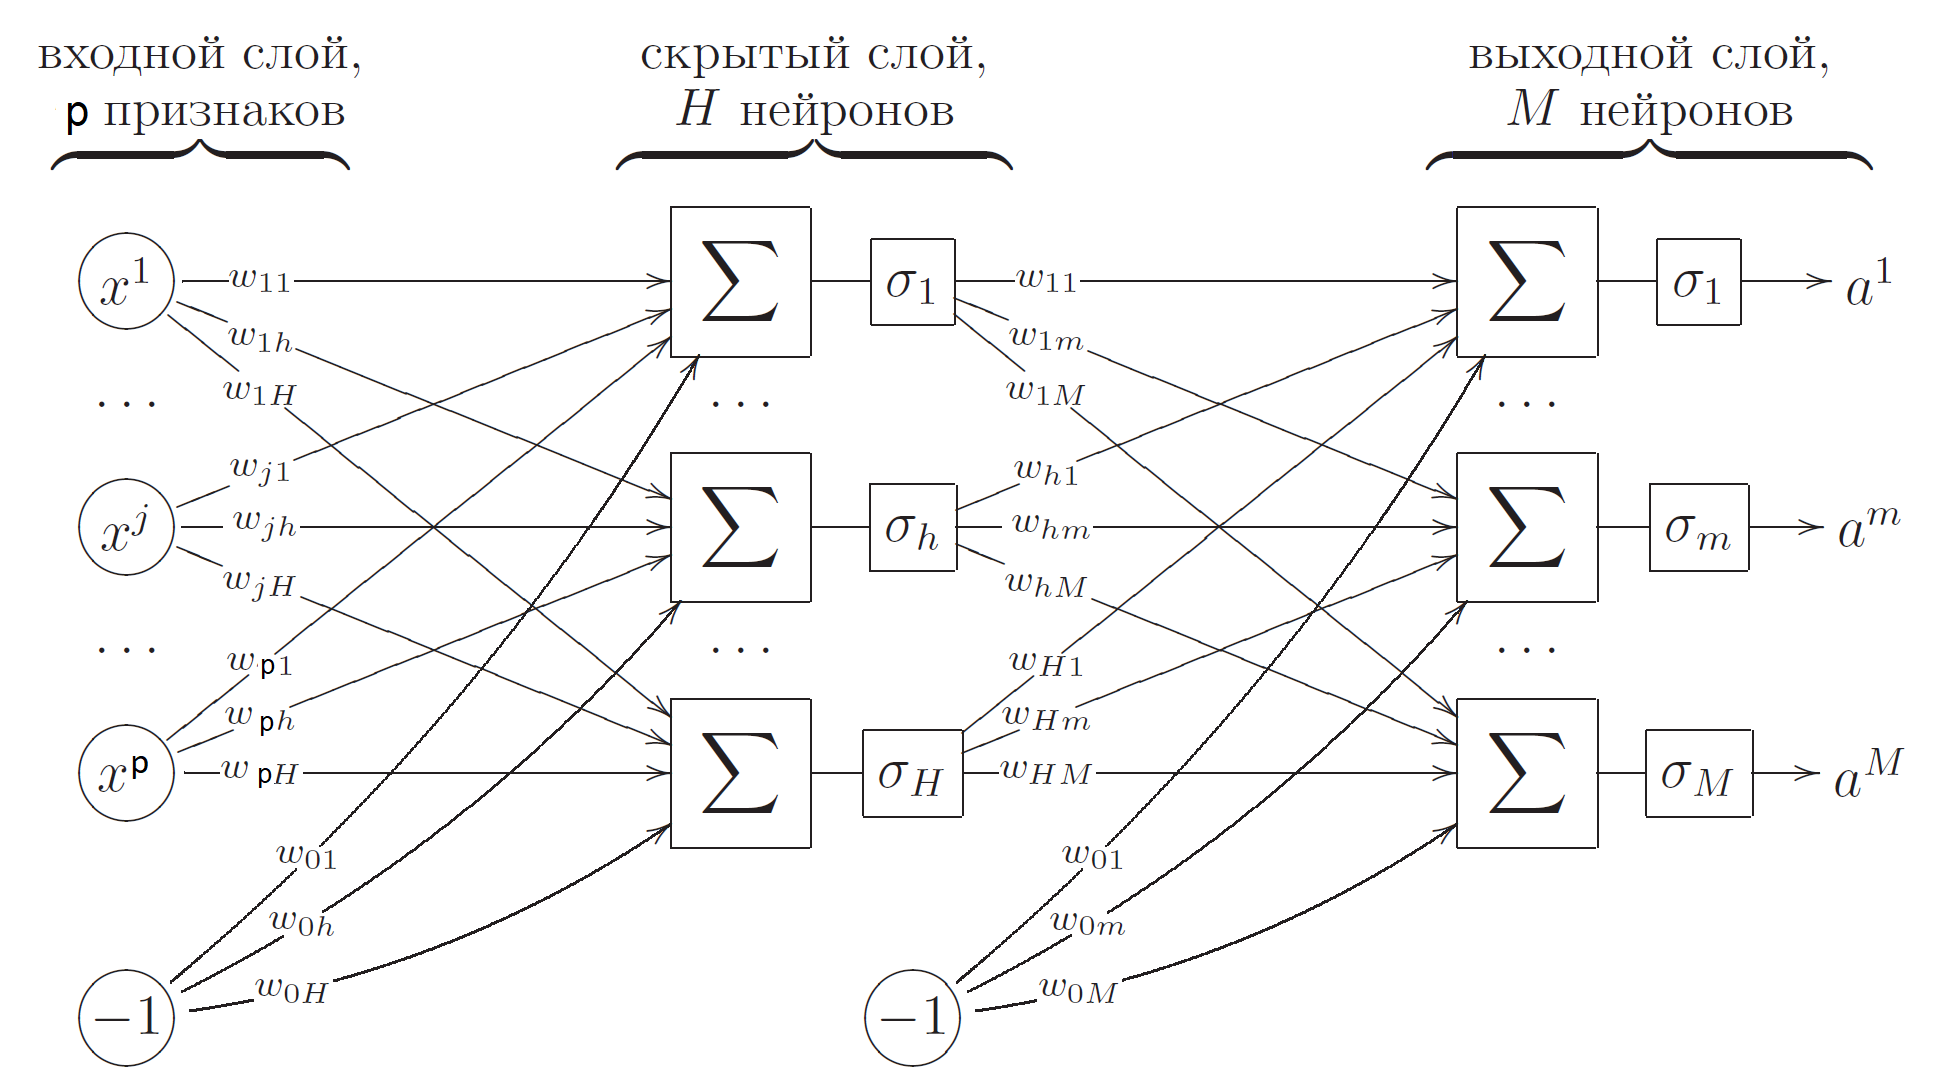
\includegraphics[width=400pt, height=200pt]{neuralnetwork}
	    \caption{Двухслойная нейронная сеть}
		\label{neuralnetwork}
	\end{minipage}
\end{center}
\end{figure}

\textbf{Проблема:} Посчитаем число параметров в такой модели. В случае двухслойной нейронной сети получим $(p+1)H+(H+1)M$ весовых коэффициентов. Для решения поставленной задачи используются градиентные методы, в частности, стохастический градиентный спуск, однако при таком большом количестве параметров посчитать градиент довольно трудоемко. Для решения этой проблемы возник метод обратного распространения ошибки, который с некоторыми затратами памяти эффективно вычисляет градиент.

Для начала поставим промежуточную задачу эффективного вычисления частных производных $\frac{\partial \mathcal{L}_i(w)}{\partial a^m}$ и $\frac{\partial \mathcal{L}_i(w)}{\partial u^h}$. Идея состоит в том, что при первом вычислении сети мы будем сохранять некоторые величины, которые впоследствии помогут быстро посчитать градиент.

В случае двухслойной сети: $a^m(x_i)$, $m=1,\ldots,M$ на объекте $x_i$:
\begin{equation*}
a^m(x_i) = \sigma_m \left(\sum_{h=0}^{H} w_{hm}  u^h(x_i)  \right), ~~~~~~
 u^h(x_i) = \sigma_h \left(\sum_{j=0}^{p} w_{jh} x_{i}^j   \right).
\end{equation*}
Пусть для конкретности
\begin{equation*}
\mathcal{L}_i(w) = \frac{1}{2} \sum_{m=1}^{M}(a^m(x_i) - y^m_i)^2,
\end{equation*}
для других функций потерь рассуждения можно провести по аналогии.

Выпишем выражения для частных производных. Для краткости записи будем обозначать $\sigma'_m = \sigma'_m (\sum\limits_{h=0}^H w_{hm} u^h(x_i))$ и аналогично для других производных в соответствующих точках.
\begin{equation*}
\frac{\partial \mathcal{L}_i(w)}{\partial a^m} = a^m(x_i) - y_i^m = \varepsilon^m_i ~~\text{ --- ошибка на выходном слое,}
\end{equation*}

\begin{equation*}
\frac{\partial \mathcal{L}_i(w)}{\partial u^h} = \sum \limits_{m=1}^M (a^m(x_i) - y_i^m) \sigma_m' w_{hm} = \sum \limits_{m=1}^M \varepsilon^m_i \sigma_m' w_{hm} = \varepsilon^h_i.
\end{equation*}
По аналогии назовем это также ошибкой на нейроне промежуточного слоя.

Теперь заметим, что $\varepsilon_i^h$ вычисляется по $\varepsilon_i^m$, если запустить сеть в обратном порядке, справа налево:

	\begin{center}
	\begin{minipage}{0.51\linewidth}
		\centering
		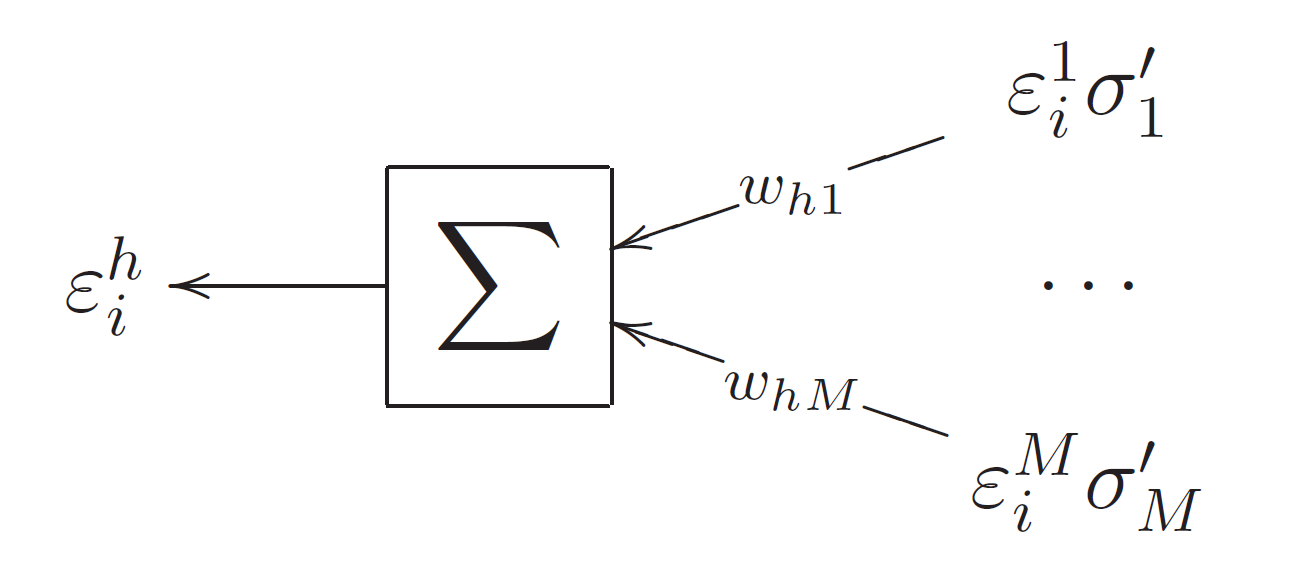
\includegraphics[width=220pt, height=100pt]{backprop}
		%\captionof{figure}{}
	\end{minipage}
\end{center}

Итак, имеем формулы для компонент вектора градиента:
\begin{equation*}
\frac{\partial \mathcal{L}_i(w)}{\partial w_{hm}} = \frac{\partial \mathcal{L}_i(w)}{\partial a^m} \frac{\partial a^m}{\partial w_{hm}} =   \varepsilon^m_i \sigma_m' u^h(x_i), ~~~~~ h=0,\ldots,H, ~~ m=1,\ldots,M,
\end{equation*}

\begin{equation*}
\frac{\partial \mathcal{L}_i(w)}{\partial w_{jh}} = \frac{\partial \mathcal{L}_i(w)}{\partial u^h} \frac{\partial u^h}{\partial w_{jh}} =   \varepsilon^h_i \sigma_h' f_j(x_i), ~~~~~ j=0,\ldots,p, ~~ h=1,\ldots,H.
\end{equation*}

Будем сохранять промежуточные величины $\varepsilon_i^m$ и $\varepsilon_i^h$, чтобы эффективно вычислить компоненты вектора градиента. Полученный алгоритм --- это метод стохастического градиентного спуска с быстрым вычислением градиента. \\

\begin{algorithm}[H]
	\SetAlgoLined
	\KwIn{$\mathbb{X}^n=\{x_i, y_i\}_{i=1}^n$ --- обучающая выборка, $x_i \in \mathbb{R}^p$, $y_i \in \mathbb{R}^M$, $H$ --- число нейронов на скрытом слое, $\eta$ --- темп обучения, параметр $\lambda$}
	\KwOut{$w_{jh}, w_{hm}$ --- веса}
	
	Инициализация весов $w_{jh},~ w_{hm}$\;
	\Repeat{$Q$ не сойдется}{
		Выбираем $x_i$ из $\mathbb{X}^n$\;
		Прямой ход: ~~~~~~~~~~~~~~~~~~~~~~~~~~~~~~~~~~~~~~~~~~~~~~
		$u^h:=\sigma_h(\sum\limits_{j=0}^n w_{jh}x_i^j), ~~~ h=1,\ldots,H$;
		$a^m:=\sigma_m(\sum\limits_{h=0}^H w_{hm}u_i^h),~~ \varepsilon_i^m:=a_i^m-y_i^m, ~~~ m=1,\ldots,M$; ~~~~~~~~~~~~~~
		$\mathcal{L}_i:=\sum\limits_{m=1}^M (\varepsilon_i^m)^2$ \;
		Обратный ход: $\varepsilon_i^h:= \sum\limits_{m=1}^M \varepsilon_i^m\sigma_m' w_{hm}, ~~~ h=1,\ldots,H$\;
		Градиентный шаг: 
		$w_{hm}:=w_{hm}-\eta \varepsilon_i^m \sigma_m' u^h(x_i), ~~~~~~ h=0,\ldots,H, ~ m=1,\ldots,M$;
		$w_{jh}:=w_{jh}-\eta \varepsilon_i^h \sigma_h' f^j(x_i), ~~~~~~ j=0,\ldots,p, ~ h=1,\ldots,H$ \;
		$Q:=(1-\lambda)Q+\lambda\mathcal{L}_i$;		
	}
	\caption{обучение двухслойной нейронной сети методом обратного распространения ошибки (back-propagation)}
\end{algorithm}
~~~\\
~~~\\
~~~ \\

\textbf{Достоинства} метода обратного распространения ошибок:
\begin{itemize}
	\item эффективность: быстрое вычисление градиента. В случае двухслойной сети прямой ход, обратный ход и вычисление градиента требуют порядка $O(Hp+HM)$ операций;
	\item метод легко обобщается на любые функции потерь, функции активации, произвольное количество слоев и произвольную размерность входов и выходов;
	\item возможно динамическое (потоковое) обучение;
	\item на сверхбольших выборках не обязательно брать все $x_i$.
\end{itemize}

\textbf{Недостатки} (есть все те же, что и у метода стохастического градиента):
\begin{itemize}
	\item метод не всегда сходится;
	\item возможна медленная сходимость;
	\item застревание в локальных минимумах;
	\item проблема переобучения.
\end{itemize}

\section{Некоторые способы улучшения сходимости}

Для улучшения сходимости применимы некоторые эвристики:
	\begin{enumerate}
	\item инициализация весов;
	\item порядок предъявления объектов;
	\item оптимизация величины градиентного шага;
	\item регуляризация (сокращение весов). 
\end{enumerate} 

\textbf{Инициализация весов.} 
Есть несколько вариантов выбора начальных весов. Рассмотрим некоторые из них.
\begin{enumerate}
\item Часто веса инициализируются случайно, небольшими по модулю значениями. Например, в качестве начального приближения берутся случайные значения из отрезка $[-\frac{1}{2k}, \frac{1}{2k}]$, где $k$ --- число нейронов в том слое, из которого выходит связь.
\item Существует вариант инициализации весов в зависимости от корреляции признака и столбца ответов:
\begin{equation*}
w_{jh}=\frac{\langle x^j, y\rangle}{\langle x^j, x^j\rangle} + \varepsilon_{jh}.
\end{equation*}
В таком случае чем больше похожи $x^j$ и $y$, тем больше вес. Чтобы веса не инициализировались одинаково, к ним добавляется некоторая случайность. 

\item Начальное приближение также можно сформировать по-другому. Идея заключается в том, чтобы сначала настроить нейроны первого слоя отдельно, как H однослойных нейронных сетей. Затем по-отдельности настраиваются нейроны второго слоя, которым на вход подаётся вектор выходных значений первого слоя. Чтобы сеть не получилась вырожденной, нейроны первого слоя должны быть существенно различными. Будет хорошо, если они будут хоть как-то приближать целевую зависимость, тогда второму слою останется только усреднить результаты первого слоя, сгладив ошибки некоторых нейронов. Для этого необходимо обучать нейроны первого слоя на различных случайных подвыборках, либо подавать им на вход различные случайные подмножества признаков. Так как при формировании начального приближения не требуется особая точность, поэтому отдельные нейроны можно обучать простейшими градиентными методами.

\end{enumerate}

\textbf{Выбор градиентного метода.} Из-за того, что градиентные методы первого порядка сходятся довольно медленно, они редко применяются на практике. Ньютоновские методы второго порядка также непрактичны, потому что они требуют вычисления матрицы вторых производных функционала $Q(w)$, имеющей слишком большой размер. Поэтому можно использовать следующие варианты улучшения сходимости.
\begin{enumerate}
	\item \textbf{Метод стохастического градиента с адаптивный шагом.} Идея заключается в том, что на каждом шаге подбирается параметр $\eta_{*}$:
	\begin{equation*}
		Q(w - \eta \frac{\delta Q}{\delta w}) \rightarrow \min_\eta.
	\end{equation*}
	
	Для решения этой задачи не обязательно находить точный минимум, поэтому можно использовать простейшие методы оптимизации.
	\item \textbf{Диагональный метод Левенберга-Марквардта.}
		В методе Ньютона-Рафсона второго порядка:
	\begin{equation*}
	w := w - \eta (Q^{''}(w))^{-1} Q^{'}(w),
	\end{equation*}
	где $Q^{''}(w) = \left( \frac{\partial^2 Q(w) }{\partial w_{jh} \partial w_{j^{'}h^{'}}}   \right)$ --- гессиан размера $(H(p+M+1) + M)^2$.
	
	Эвристика состоит в том, что мы считаем, что гессиан диагонален:
	\begin{equation*}
	w_{jh} := w_{jh} - \eta \left(  \frac{\partial^2 Q(w) }{\partial w_{jh}^2} + \mu  \right) ^{-1} \frac{\partial Q(w) }{\partial w_{jh}}, 
	\end{equation*} 
	$\mu$ --- параметр, предотвращающий обнуление знаменателя, \\
	$\frac{\eta}{\mu}$ --- темп обучения на ровных участках функционала $Q(w)$, где вторая производная равна нулю.
	
	~~~~~~Данный метод является неким усреднением методов первого порядка и второго порядка. Методы 1-ого порядка плохо сходятся вблизи окрестности минимума, там функция плохо приближается линейной, но хорошо приближается квадратичной. Метод Левенберга-Марквардта быстрее сходится в окрестности минимума из-за того, что учитываются вторые производные. Таким образом, метод Левенберга-Марквардта вблизи точки минимума похож на метод 2-ого порядка, а вдали --- на метод 1-ого порядка.
\end{enumerate}

\section{Выбор структуры нейронной сети}

Выбор структуры сети заключается в выборе числа слоёв, числа нейронов и числа связей для каждого нейрона. Существуют различные стратегии поиска оптимальной структуры сети, например, постепенное наращивание или построение заведомо слишком сложной сети с последующим упрощением. Мы рассмотрим эти варианты далее.

Неправильный выбор структуры сети приводит к проблемам недообучения и переобучения. Понятно, что слишком простые сети не способны адекватно моделировать целевые зависимости в реальных задачах. Слишком сложные сети имеют избыточное число свободных параметров, которые в процессе обучения настраиваются не только на восстановление целевой зависимости, но и на воспроизведение шума.

\textbf{Выбор числа слоёв.} Если знаем, что классы линейно разделимы, то нам достаточно ограничиться одним слоем. Если граница между классами нелинейная и извилистая, то в большинстве случаев достаточно взять двухслойную сеть. Трёхслойными сетями имеет смысл пользоваться для представления сложных многосвязных областей. Теоретически, можно взять нейронную сеть с большим количеством слоев, однако тогда хуже сходятся градиентные методы, и тем труднее нам будет её обучить.

\textbf{Выбор числа нейронов в скрытом слое (выбор H).} Имеется несколько способов выбора числа нейронов в скрытых слоях.
\begin{enumerate}
	\item Визуальный способ. Если граница классов (или кривая регрессии) слишком сглажена --- количество нейронов в слое нужно увеличить, а если есть резкие колебания, то, наоборот, уменьшить. Этот способ подходит для задач с небольшим числом признаков.
	\item По внешнему критерию. Можно смотреть на среднюю ошибку на тестовой выборке или использовать cross-validation. Недостаток этого способа --- высокая трудоёмкость. Приходится много раз заново строить сеть при различных значениях параметра $H$, а в случае скользящего контроля --- ещё и при различных разбиениях выборки на обучающую и контрольную части.
\end{enumerate}

\textbf{Динамическое наращивание сети.} Состоит в следующих шагах:


\begin{enumerate}
	\item Обучение сети при заведомо недостаточном числе нейронов $H \ll n$, пока ошибка не перестаёт убывать;
	\item Добавление нового нейрона и его инициализация путем обучения 
	\begin{itemize}
		\item либо по случайной подвыборке $X^{'} \subseteq X^n$;
		\item либо по объектам с наибольшими значениями потерь;
		\item либо по случайному подмножеству входов;
		\item либо из различных случайных начальных приближений.
	\end{itemize}
	\item Снова итерации BackProp;
\end{enumerate}


Эмпирический опыт заключается в том, что после добавления новых нейронов ошибка, обычно, сначала резко возрастает, затем быстро сходится к меньшему значению. Общее время обучения обычно лишь в $1.5$--$2$ раза больше, чем если бы в сети сразу было нужное количество нейронов. Полезная информация, накопленная сетью, не теряется при добавлении новых нейронов. Также полезно наблюдать за внешним критерием: прохождение $Q(X^k)$ через минимум является надежным критерием останова.


\textbf{Удаление избыточных связей (OBD --- Optimal Brain Damage).} Идея заключается в удалении тех связей, к изменению которых функционал $Q(w)$ наименее чувствителен. Уменьшение числа весов снижает склонность сети к переобучению.

Пусть $w$ --- локальный минимум $Q(w)$, тогда $Q(w)$ можно аппроксимировать квадратичной формой по формуле Тейлора:
\begin{equation*}
Q(w + \delta) = Q(w) + \frac{1}{2} \delta^{\mathrm{T}} Q^{''}(w) \delta + o(\| \delta\|^2),
\end{equation*}
где $Q^{''}(w) =  \frac{\partial^2 Q(w) }{\partial w_{jh} \partial w_{j^{'}h^{'}}}$ --- гессиан размера $(H(p+M+1) + M)^2$.\\

Пусть гессиан $Q^{''}(w)$ диагонален, тогда
\begin{equation*}
\delta^{\mathrm{T}} Q^{''}(w) \delta = \sum_{j=0}^{p}\sum_{h=0}^{H} \delta^2_{jh}   \frac{\partial^2 Q(w) }{\partial w_{jh}^2 }  +  \sum_{h=0}^{H}\sum_{m=0}^{M} \delta^2_{hm}   \frac{\partial^2 Q(w) }{\partial w_{hm}^2 }.
\end{equation*}
Хотим обнулить вес, это эквивалентно условию $w_{jh} + \delta_{jh}=0$. Определим \textit{значимость (salience)} веса $w_{jh}$ как изменение функционала $Q(w)$ при его обнулении: $S_{jh} = w^2_{jh}  \frac{\partial^2 Q(w) }{\partial w_{jh}^2 } $. Делаем следующие шаги:

\begin{enumerate}
\item В BackProp вычисляем вторые производные $\frac{\partial^2 Q(w) }{\partial w_{jh}^2 } $,  $\frac{\partial^2 Q(w) }{\partial w_{hm}^2 } $.
\item Если процесс минимизации $Q(w)$ пришел в минимум, то
\begin{itemize}
\item упорядочиваем веса по убыванию $S_{jh}$;
\item удаляем $d$ связей с наименьшей значимостью;
\item снова запускаем BackProp.
\end{itemize}
\item Если $Q(w, X^n)$ или $Q(w, X^k)$ существенно ухудшился, то необходимо вернуть последние удаленные связи и выйти.
\end{enumerate}

Аналогично, OBD можно использовать для отбора информативных признаков для нейрона скрытого слоя.
Суммарная значимость признака: $S_j = \sum_{h=1}^{H} S_{jh}$. Из сети удаляем один или несколько признаков с наименьшей $S_j$.

Эмпирический опыт: сеть, построенная с помощью OBD, меньше склонна к переобучению, чем сеть сразу построенная по полученной структуре (со случайно инициализированными весами).


\end{document}